\section{Introduction}
In 1978, Thomas C. Schelling developed his tipping model by placing pennies and dimes on a chess board and moved them according to various rules. 
By viewing the pennies and dimes as two types of people, the rule of moving as a preference for the individuals, and the chess board as a city, he soon discovered that segregation is formed on the board, even when the preference of the individuals is very subtle.\\
\\
Based on this idea, we first built a basic model which consists of an $8\times8$ board with $40$ individuals that are divided in two types. 
The individuals are moved according to their 'Happiness' in the current place. 
For the basic model, an individual is considered happy if $\frac{1}{3}$ of his/her second order neighbours (a person has at most $8$ neighbours) is of the same type. 
Otherwise, an individual is considered unhappy and will be moved to the nearest place such that his/her happiness is strictly higher, which will be referred to as the 'Happiness Rule'. 
For example, we can see that not all individuals in figure \ref{fig:ebmb} are happy and after segregation they are located like figure \ref{fig:ebme}.

\begin{figure}[H]
	\centering
    \begin{subfigure}{0.45\textwidth}
        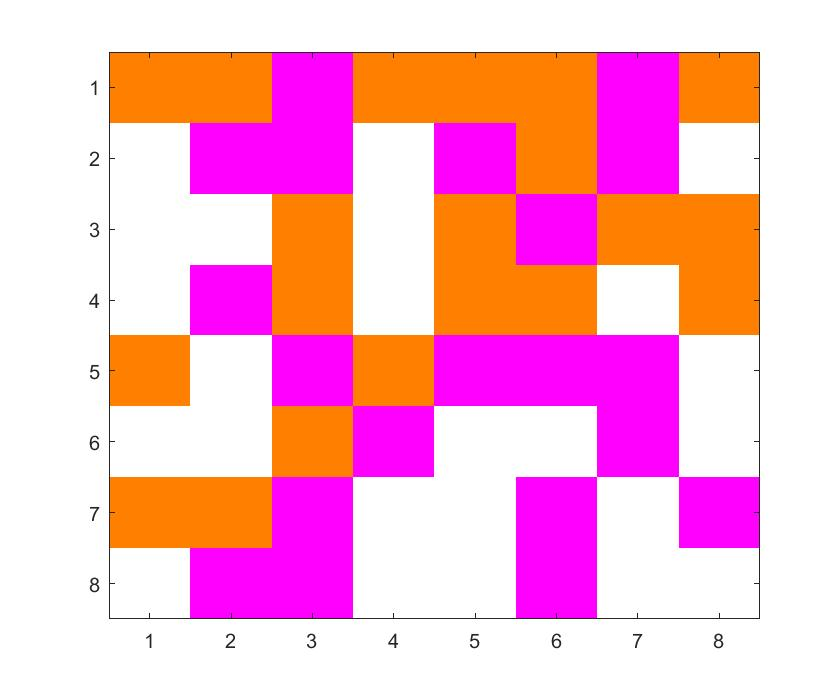
\includegraphics[width=\textwidth]{vb1beginbord.jpg}
        \caption{Situation before segragation}
        \label{fig:ebmb}
    \end{subfigure}\hspace{0cm}
    ~ %add desired spacing between images, e. g. ~, \quad, \qquad, \hfill etc. 
      %(or a blank line to force the subfigure onto a new line)
    \begin{subfigure}{0.45\textwidth}
        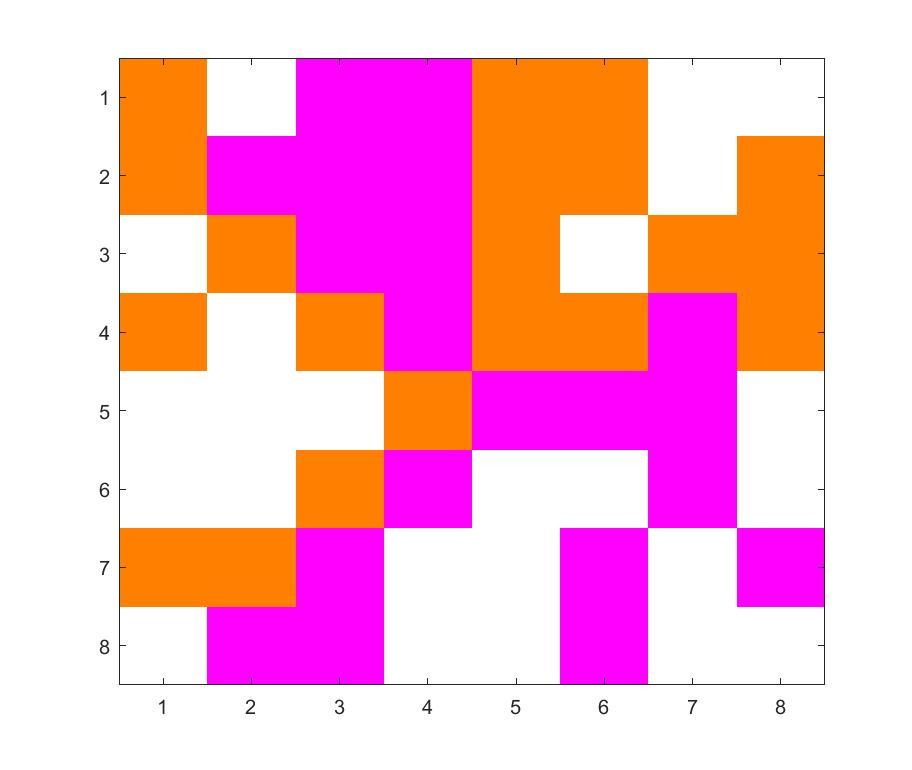
\includegraphics[width=\textwidth]{vb1eindbord.jpg}
        \caption{Situation after segregation}
        \label{fig:ebme}
    \end{subfigure}
    ~ %add desired spacing between images, e. g. ~, \quad, \qquad, \hfill etc. 
    %(or a blank line to force the subfigure onto a new line)
    \caption{An example of segregation in our basic model: type 1 is orange and type 2 is pink}
    \label{fig:example basic model}
\end{figure}

After that, we extended the basic model by changing the parameters such as the size of the population, board and number of types. 
We also included an option for random displacement: an individual which is not happy will be moved to a empty location randomly. 
(That is to say, that individual will be placed to any empty spot with equal probability.)

For both the basic and the extended model, we ran $500$ simulations several times and investigated how different values of the parameters affected the segregation pattern. 
In order to formulate our research goals precisely, the following definitions are important:\\
1. \textbf{Generation}: 
A population is said to have entered a next generation if the happiness of every individual has been checked once. \\
2. \textbf{Equilibrium}: 
The population is said to have reached an equilibrium if there are no individuals that have moved in the past generation.\\
3. \textbf{Segregation time at $n\%$}: 
The segregation time at $n\%$ is defined as the number of generations such that $n\%$ of the population has all his/her neighbours of the same type.\\

For this project, we focussed on the following main questions:\\
1. How do the parameters affect the equilibrium? 
Does the population always reach an equilibrium? 
How many generations on average does it take to reach an equilibrium? 
What's the probability distribution of the number of generations to reach an equilibrium?\\
2. What fraction of the individuals is happy after the equilibrium? 
Can we optimize that by changing the size of the bord?\\
3. What is the segregation time for 60$\%$ and how does the definition of the happiness affect it?\\
\\
Short abstract about main findings...\\
how the report looks like further on...